\documentclass[12pt]{article}
\usepackage[utf8]{inputenc}
\newcommand\preamble{
    \usepackage[italian]{babel}
    \usepackage{geometry}
    \usepackage{amsmath}
    \usepackage{amssymb}
    \usepackage{graphicx}
    \usepackage{ulem}
    \usepackage[dvipsnames]{xcolor}

    \geometry{margin=2cm}
    \let\olditemize\itemize
    \renewcommand\itemize{\olditemize\setlength\itemsep{0em}}
    \graphicspath{{../Immagini/}}

    \author{Lorenzo Vaccarecci}
}
\preamble

\title{Ottimizzazione Fisica}
\date{19 Aprile 2024}

\begin{document}
\maketitle
\section{Introduzione}
\begin{itemize}
    \item \textbf{Input}: piano di esecuzione logica ottimizzato
    \item \textbf{Output}: piano di esecuzione fisico ottimale (PQP)
\end{itemize}
\textcolor{red}{Piano di esecuzione fisico}: algoritmo di esecuzione dell'interrogazione, rappresentato come albero, sul livello fisico.
\subsection{Esempio}
Ogni nodo corrisponde a un algoritmo
\begin{center}
    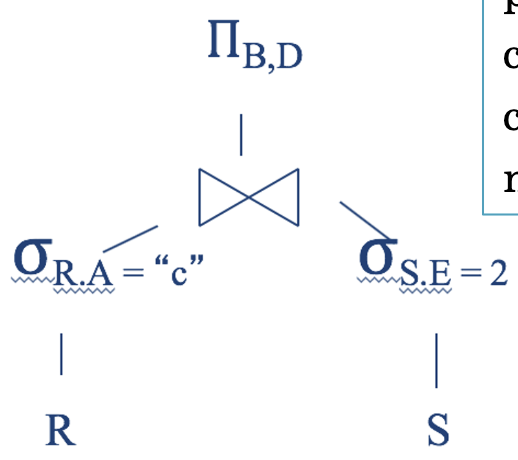
\includegraphics[scale=0.6]{esempioalberolivellofisico.png}
    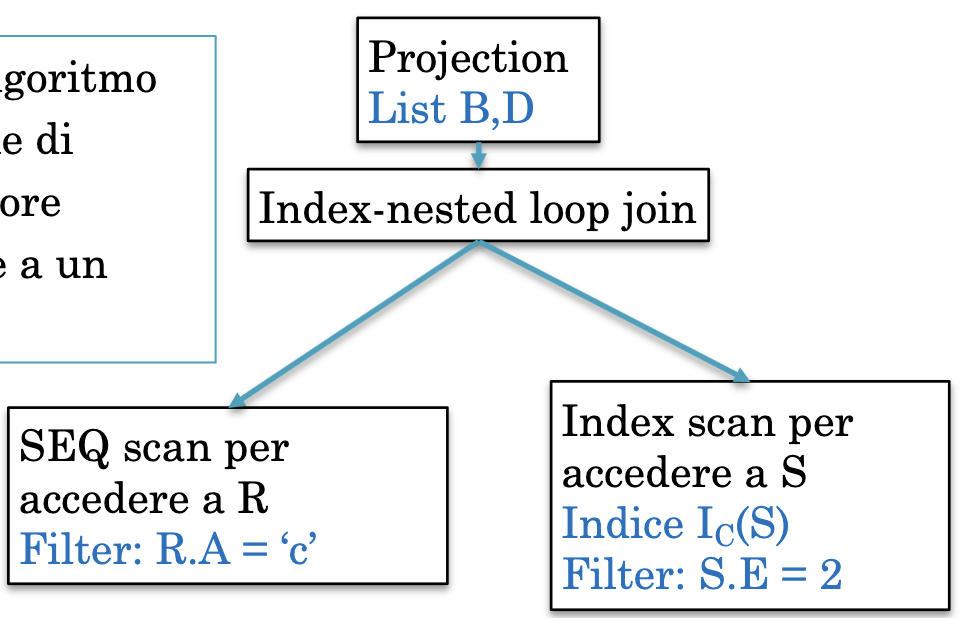
\includegraphics[scale=0.6]{esempioalberofisico.png}
\end{center}
\textbf{Schema fisico}
\begin{itemize}
    \item File per $R$ ordinato rispetto ad $A$
    \item File per $S$ ordinato rispetto ad $C$
    \item Indice ordinato su $R.A:I_{A}(R)$
    \item Indice ordinato su $S.C:I_{C}(S)$
\end{itemize}
\end{document}